\chapterhead{CHƯƠNG 3 $-$ CHỨNG THỰC TRONG VPN}
\addcontentsline{toc}{chapter}{CHƯƠNG 3 $-$ CHỨNG THỰC TRONG VPN}
\vspace{-0.5cm}

Để xác thực và bảo vệ dữ liệu trong hệ thống VPN, nhiều phương pháp chứng thực đã được phát triển và áp dụng, tùy thuộc vào yêu cầu cụ thể của từng ứng dụng. Các phương pháp này đóng vai trò quan trọng trong việc đảm bảo rằng chỉ những người dùng hoặc thiết bị được ủy quyền mới có thể truy cập mạng. Mỗi phương pháp đều có những ưu điểm nổi bật và hạn chế riêng, từ mức độ bảo mật, tính linh hoạt đến sự phức tạp khi triển khai. Việc lựa chọn phương pháp phù hợp đòi hỏi phải cân nhắc giữa nhu cầu bảo mật, khả năng tích hợp và các rủi ro tiềm ẩn trong hệ thống.
 
\section*{3.1 Phương pháp PAP}
 \addcontentsline{toc}{section}{3.1 Phương pháp PAP}
 \subsection*{3.1.1 Khái quát phương pháp PAP}
 \addcontentsline{toc}{subsection}{3.1.1 Khái quát phương pháp PAP}

PAP là phương pháp xác thực giao thức PPP sử dụng mật khẩu để xác thực người dùng. Đây là một tiêu chuẩn internet (RFC 1334), giao thức xác thực dựa trên mật khẩu. Mặc dù không được xem là an toàn cao do mật khẩu được truyền đi dưới dạng văn bản rõ, nhưng PAP vẫn được sử dụng trong một số trường hợp nhất định.

 \subsection*{3.1.2 Quy tắc xác thực}
 \addcontentsline{toc}{subsection}{3.1.2 Quy tắc xác thực}

Bước 1: Khởi tạo Kết Nối.
    \begin{itemize}[left=1.5cm]
        \item Client gửi một gói tin tới máy server, yêu cầu thiết lập kết nối VPN. Gói tin này bao gồm tên người dùng.
        \item Server nhận được yêu cầu từ client và bắt đầu quá trình xác thực.
    \end{itemize}
    
Bước 2: Gửi Challenge

\begin{itemize}[left=1.5cm]
        \item Server Tạo Challenge: Server tạo ra một chuỗi ký tự ngẫu nhiên, gọi là "challenge" và sau đó sẽ gửi challenge này đến client. Challenge này đóng vai trò như một câu hỏi để kiểm tra tính hợp lệ của thông tin mà client cung cấp
    \end{itemize}
    
Bước 3: Client Trả Lời
\begin{itemize}[left=1.5cm]
        \item Client nhận được challenge từ server. Sau đó, client sẽ kết hợp challenge này với mật khẩu đã lưu trữ và thực hiện một phép tính đơn giản (thường là một hàm băm) để tạo ra một kết quả, gọi là "response". Sau đó Client gửi response này trở lại cho server.
    \end{itemize}

Bước 4: Server Xác Thực
    \begin{itemize}[left=1.5cm]
        \item Server nhận được response từ client và so sánh nó với kết quả mà server đã tính toán trước đó dựa trên mật khẩu của người dùng. Nếu hai kết quả trùng khớp, server sẽ xác nhận rằng client đã cung cấp thông tin đăng nhập chính xác và cho phép client kết nối đến mạng VPN. Ngược lại, nếu hai kết quả không khớp, server sẽ từ chối kết nối.
    \end{itemize}

    \begin{figure}[htbp]
        \centering
        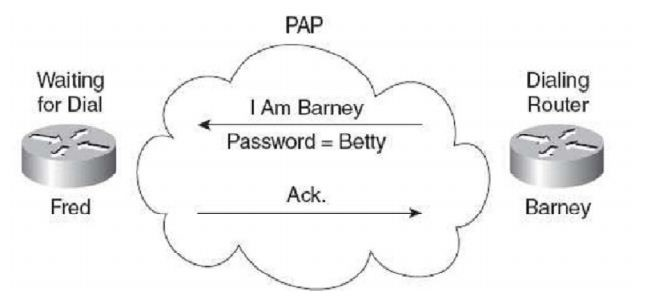
\includegraphics[width=0.7\linewidth]{img/pap.jpeg}
        \caption{Quá trình hoạt động của PAP}
        \end{figure}

 \subsection*{3.1.3 Ưu điểm}
 \addcontentsline{toc}{subsection}{3.1.3 Ưu điểm}

 Đơn giản và dễ triển khai: PAP rất đơn giản và dễ cấu hình, điều này làm cho nó trở thành một lựa chọn phổ biến trong các môi trường không yêu cầu bảo mật cao. Việc triển khai PAP không đòi hỏi phần cứng hoặc phần mềm đặc biệt, giúp tiết kiệm thời gian và chi phí.

Chi phí thấp: Vì PAP không yêu cầu các công nghệ mã hóa phức tạp hay chứng chỉ số, nên chi phí triển khai và bảo trì thấp hơn so với các phương pháp chứng thực khác, chẳng hạn như EAP hoặc CHAP.

Tương thích rộng rãi: PAP là một giao thức cũ và đã được hỗ trợ rộng rãi trên hầu hết các nền tảng và thiết bị, bao gồm các hệ thống mạng và VPN cũ. Điều này làm cho nó dễ dàng tích hợp vào các môi trường hiện có mà không cần thay đổi lớn.
 
Tốc độ xử lý nhanh: Do quy trình xác thực tương đối đơn giản, PAP có thể xử lý các yêu cầu xác thực nhanh chóng, giúp tăng hiệu suất kết nối.

 \subsection*{3.1.4 Nhược điểm}
 \addcontentsline{toc}{subsection}{3.1.4 Nhược điểm}

Mật khẩu truyền không được mã hóa: Đây là nhược điểm lớn nhất của PAP. Mật khẩu được gửi qua mạng dưới dạng văn bản rõ, rất dễ bị đánh cắp nếu bị nghe lén. Điều này làm tăng nguy cơ bị tấn công và xâm nhập trái phép.

Không an toàn: Do mật khẩu không được bảo vệ, PAP không cung cấp mức độ bảo mật cao. Nó rất dễ bị tấn công bởi các cuộc tấn công từ chối dịch vụ (DoS), tấn công replay, và các hình thức tấn công khác.

Thiếu cơ chế xác thực mạnh: PAP không có các cơ chế xác thực mạnh như mã hóa hoặc xác thực hai yếu tố, làm giảm tính tin cậy của giao thức.

Dễ bị tấn công bằng từ điển: Vì mật khẩu được truyền dưới dạng văn bản rõ, tin tặc có thể dễ dàng sử dụng các công cụ tấn công bằng từ điển để đoán mật khẩu.

 
 \section*{3.2 Phương pháp CHAP}
 \addcontentsline{toc}{section}{3.2 Phương pháp CHAP}
 \subsection*{3.2.1 Khái quát phương pháp CHAP}
 \addcontentsline{toc}{subsection}{3.2.1 Khái quát Phương pháp CHAP}
CHAP là một phương thức xác thực mạnh mẽ hơn so với PAP, được sử dụng trong các kết nối VPN hoặc các mạng dial-up. Đây là một phương thức chứng thực trong VPN giúp xác thực người dùng hoặc thiết bị kết nối một cách an toàn hơn so với PAP. Khác với PAP, CHAP không gửi mật khẩu qua mạng dưới dạng văn bản thuần. Thay vào đó, giao thức này sử dụng một cơ chế thách thức và phản hồi. Tuy nhiên, dù bảo mật hơn PAP, CHAP vẫn có thể gặp phải các vấn đề nếu mật khẩu yếu hoặc không được bảo vệ tốt.

  \subsection*{3.2.2 Quy tắc xác thực của CHAP}
 \addcontentsline{toc}{subsection}{3.2.2 Quy tắc xác thực của CHAP}

Máy chủ truy cập mạng thực hiện tra cứu tên máy chủ trên người dùng và gửi một "thử thách” cho người dùng để bắt đầu xác thực CHAP.

Sau đó, người dùng thực hiện tra cứu tên máy chủ. Người dùng sẽ sử dụng mật khẩu mà cả người dùng và máy chủ đều biết để tạo ra một hàm băm một chiều được mã hóa. Hàm băm được mã hóa này dựa trên chuỗi thử thách.

Máy chủ xác minh băm bằng cách giải mã để đảm bảo rằng nó khớp với chuỗi thử thách ban đầu. Khi các chuỗi khớp, một thông báo xác thực thành công được gửi đi và phiên PPP được thiết lập. Nếu các chuỗi không khớp, một thông báo xác thực thất bại được tạo ra và phiên bị chấm dứt.

    \begin{figure}[htbp]
        \centering
        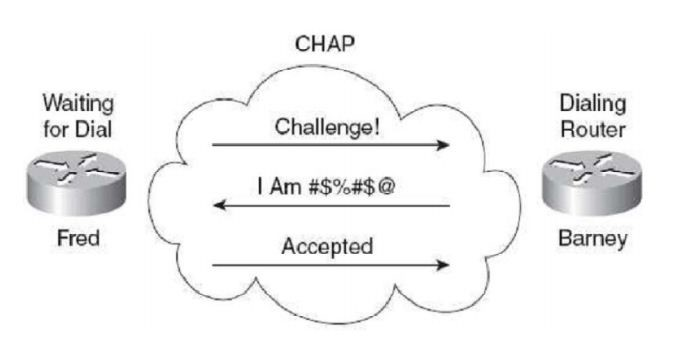
\includegraphics[width=0.7\linewidth]{img/chap.jpeg}
        \caption{Quá trình hoạt động của CHAP}
    \end{figure}

  \subsection*{3.2.3 Ưu điểm}
 \addcontentsline{toc}{subsection}{3.2.3 Ưu điểm}

 Mã hóa thông tin xác thực: Mật khẩu không được gửi trực tiếp qua mạng. Thay vào đó, giá trị băm của mật khẩu được trao đổi, giúp bảo mật hơn so với PAP.
 
Chống lại các cuộc tấn công Replay: Vì mỗi lần xác thực đều sử dụng một thách thức ngẫu nhiên khác nhau, CHAP bảo vệ kết nối khỏi các cuộc tấn công "replay" (tái sử dụng thông tin xác thực cũ).

Xác thực định kỳ: Sau khi kết nối thành công, CHAP có thể yêu cầu xác thực lại trong suốt phiên làm việc, giúp tăng cường bảo mật.


  \subsection*{3.2.4 Nhược điểm}
 \addcontentsline{toc}{subsection}{3.2.4 Nhược điểm}

Cấu hình phức tạp hơn PAP: Mặc dù bảo mật tốt hơn, việc triển khai CHAP đòi hỏi cấu hình phức tạp hơn so với PAP, và có thể yêu cầu phần cứng, phần mềm hỗ trợ chứng chỉ số hoặc các phương thức bảo mật khác.

Không hỗ trợ xác thực mạnh mẽ hơn: CHAP không hỗ trợ các phương thức xác thực mạnh mẽ hơn như xác thực đa yếu tố (2FA) hoặc sử dụng chứng chỉ số, điều này làm hạn chế khả năng bảo vệ trong các hệ thống đòi hỏi bảo mật cao.

Vẫn có nguy cơ nếu mật khẩu yếu: Mặc dù CHAP an toàn hơn PAP, nhưng nếu mật khẩu của người dùng yếu hoặc dễ đoán, hệ thống vẫn có thể bị tấn công. Tính bảo mật của CHAP phụ thuộc vào độ mạnh của mật khẩu được sử dụng.

Không hoàn toàn miễn nhiễm với tấn công brute-force: Dù CHAP sử dụng băm để bảo vệ mật khẩu, nhưng nếu thuật toán băm hoặc mật khẩu không đủ mạnh, hệ thống vẫn có thể bị tấn công bằng phương pháp brute-force, đặc biệt là nếu kẻ tấn công có đủ thời gian và tài nguyên.


 \section*{3.3 Phương pháp MS-CHAPv2}
 \addcontentsline{toc}{section}{3.3 Phương pháp MS-CHAPv2}
 \subsection*{3.3.1 Khái quát phương pháp MS-CHAPv2}
 \addcontentsline{toc}{subsection}{3.3.1 Khái quát phương pháp MS-CHAPv2}

 MS-CHAP là một phương thức xác thực cải tiến dựa trên CHAP, được Microsoft phát triển và sử dụng chủ yếu trong các môi trường Windows và các kết nối VPN với mục đích bảo vệ thông tin người dùng và đảm bảo tính toàn vẹn của dữ liệu truyền đi. Đây là một phiên bản nâng cấp của MS-CHAP, cung cấp khả năng bảo mật cao hơn và khắc phục một số hạn chế của phiên bản trước đó.

\subsection*{3.3.2 Quy tắc xác thực của MS-CHAPv2}
 \addcontentsline{toc}{subsection}{3.3.2 Quy tắc xác thực của MS-CHAPv2}

MS-CHAPv2 sử dụng một quy trình tương tự như CHAP nhưng có thêm các bước bổ sung.

Thách thức và phản hồi: Như trong CHAP, máy chủ sẽ gửi một thách thức ngẫu nhiên tới client. Tuy nhiên, thay vì chỉ sử dụng một giá trị băm của mật khẩu, MS-CHAPv2 kết hợp mật khẩu, thách thức ngẫu nhiên và một giá trị số ngẫu nhiên khác (nonce) để tạo ra các giá trị phản hồi phức tạp hơn.

Xác thực hai chiều: MS-CHAPv2 cung cấp xác thực hai chiều, có nghĩa là cả client và server đều phải xác thực lẫn nhau. 

Khởi tạo và kết thúc phiên: Quá trình xác thực bao gồm một loạt các thông điệp bảo mật để xác minh tính hợp lệ của các bên tham gia trong phiên kết nối. Khi xác thực thành công, cả client và server sẽ tạo ra một khóa chia sẻ để mã hóa các dữ liệu trao đổi.

\subsection*{3.3.3 Ưu điểm}
 \addcontentsline{toc}{subsection}{3.3.3 Ưu điểm}

Cung cấp xác thực lẫn nhau: MS-CHAPv2 cải thiện so với phiên bản đầu tiên bằng cách cung cấp xác thực hai chiều giữa máy khách và máy chủ. Điều này giúp giảm nguy cơ các cuộc tấn công giả mạo (man-in-the-middle).

Hỗ trợ rộng rãi: MS-CHAPv2 được Microsoft thiết kế và hỗ trợ tốt trên các hệ điều hành Windows, đồng thời được sử dụng phổ biến trong các giao thức như PPTP và trong các giải pháp VPN doanh nghiệp.

Tích hợp mã hóa: MS-CHAPv2 sử dụng khóa mã hóa được tạo trong quá trình xác thực để hỗ trợ các giao thức bảo mật khác như MPPE, đảm bảo bảo mật dữ liệu sau khi xác thực.

Khả năng triển khai nhanh: So với các giao thức yêu cầu cấu hình phức tạp như EAP-TLS, MS-CHAPv2 dễ triển khai hơn và không yêu cầu quản lý chứng chỉ số, giúp tiết kiệm thời gian

Hỗ trợ thay đổi mật khẩu từ xa: MS-CHAPv2 hỗ trợ thay đổi mật khẩu một cách an toàn ngay cả khi người dùng không có quyền truy cập trực tiếp vào hệ thống quản lý mật khẩu, giúp tăng cường trải nghiệm người dùng.

\subsection*{3.3.4 Nhược điểm}
 \addcontentsline{toc}{subsection}{3.3.4 Nhược điểm}

Bảo mật không đủ mạnh: MS-CHAPv2 sử dụng thuật toán mã hóa DES, vốn được coi là lỗi thời và dễ bị tấn công. Trong thực tế, các công cụ tấn công như Asleap có thể khai thác lỗ hổng này để bẻ khóa mật khẩu.

Phụ thuộc vào mật khẩu mạnh: Hiệu quả bảo mật của MS-CHAPv2 phụ thuộc nhiều vào độ mạnh của mật khẩu. Nếu mật khẩu yếu hoặc dễ đoán, giao thức này dễ bị tấn công brute force hoặc dictionary attack.

Không cung cấp xác thực cấp cao: So với các giao thức hiện đại như EAP-TLS, MS-CHAPv2 không hỗ trợ xác thực dựa trên chứng chỉ hoặc phương pháp sinh trắc học, làm hạn chế khả năng ứng dụng trong các hệ thống yêu cầu bảo mật cao.

Không kháng lại các tấn công nâng cao: MS-CHAPv2 không đủ mạnh để chống lại các cuộc tấn công nâng cao như tấn công offline hoặc tấn công phân tích mật khẩu dựa trên từ khóa.

Phụ thuộc vào các giao thức khác: MS-CHAPv2 không tự cung cấp mã hóa dữ liệu và phụ thuộc vào các giao thức vận chuyển (như PPTP hoặc L2TP) để bảo vệ dữ liệu, điều này làm tăng rủi ro bảo mật nếu giao thức đi kèm không đủ mạnh.

 \section*{3.4 Phương pháp EAP }
 \addcontentsline{toc}{section}{3.4 Phương pháp EAP}
 \subsection*{3.4.1 Khái quát phương pháp EAP }
 \addcontentsline{toc}{subsection}{3.4.1 Khái quát phương pháp EAP }

EAP là một phương thức linh hoạt được sử dụng để hỗ trợ nhiều phương thức xác thực trong các môi trường mạng, bao gồm cả VPN. Đây là một giao thức xác thực mở rộng, được thiết kế để cung cấp một khung làm việc linh hoạt cho các phương pháp xác thực khác nhau. Thay vì giới hạn ở một phương pháp xác thực duy nhất, EAP cho phép sử dụng nhiều loại cơ chế xác thực khác nhau, từ các phương pháp đơn giản như mật khẩu đến các phương pháp phức tạp hơn như chứng chỉ số.

  \subsection*{3.4.2 Quy tắc xác thực của EAP }
 \addcontentsline{toc}{subsection}{3.4.2 Quy tắc xác thực của EAP}

Khởi tạo: Giao thức bắt đầu khi máy khách yêu cầu quyền truy cập mạng.

Trao đổi yêu cầu/phản hồi: Máy chủ gửi yêu cầu xác thực đến máy khách, sau đó máy khách trả lời bằng thông tin danh tính.

Đàm phán phương thức: Máy chủ chọn phương thức xác thực phù hợp dựa trên cấu hình mạng và thông tin từ máy khách.

Thực hiện phương thức: Quá trình xác thực diễn ra tùy thuộc vào phương thức được chọn, ví dụ: sử dụng chứng chỉ số, mật khẩu, hoặc thông tin khác.

Xác thực hai chiều (nếu có): Một số phương thức, như EAP-TLS, cho phép cả máy chủ và máy khách xác thực lẫn nhau để đảm bảo tính bảo mật cao hơn.

Hoàn thành xác thực: Nếu thành công, máy chủ gửi thông báo "Thành công"; nếu thất bại, thông báo "Thất bại" được gửi lại.

Cấp quyền truy cập: Khi xác thực thành công, máy khách được phép truy cập tài nguyên mạng.
    \begin{figure}[htbp]
        \centering
        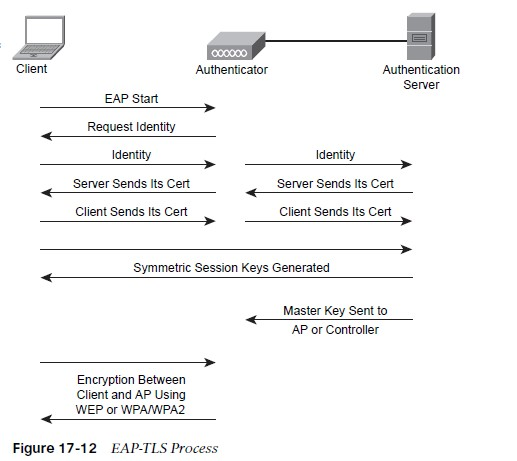
\includegraphics[width=0.6\linewidth]{img/EAP-TLS-Process.jpeg}
        \caption{Quá trình hoạt động của EAP}
    \end{figure}

\subsection*{3.4.3 Ưu điểm}
 \addcontentsline{toc}{subsection}{3.4.3 Ưu điểm}

 Tính linh hoạt cao: EAP hỗ trợ nhiều phương pháp xác thực khác nhau như mật khẩu, chứng chỉ số, thẻ thông minh, sinh trắc học, hoặc các cơ chế dựa trên token. Điều này giúp đáp ứng đa dạng các yêu cầu bảo mật và phù hợp với nhiều môi trường khác nhau.

 Mở rộng dễ dàng: Với thiết kế mô-đun, EAP cho phép thêm các phương pháp xác thực mới mà không cần thay đổi giao thức cơ bản. Đây là một lợi thế lớn khi công nghệ xác thực liên tục phát triển.
 
 Tích hợp tốt trong mạng không dây: EAP được sử dụng phổ biến trong các mạng Wi-Fi (như WPA/WPA2 Enterprise) để cung cấp xác thực an toàn giữa thiết bị và mạng, cải thiện bảo mật so với các phương pháp dựa trên mật khẩu đơn giản.

 Bảo mật nâng cao: Một số phương pháp EAP, như EAP-TLS, cung cấp xác thực lẫn nhau giữa máy khách và máy chủ, đảm bảo không có sự xâm nhập từ bên thứ ba.

 Hỗ trợ nhiều giao thức vận chuyển: EAP có thể hoạt động trên nhiều giao thức vận chuyển như PPP, 802.1X và RADIUS, làm tăng khả năng tương thích trong các hệ thống mạng khác nhau.


 \subsection*{3.4.4 Khuyết điểm}
 \addcontentsline{toc}{subsection}{3.4.4 Khuyết điểm}

 Độ phức tạp trong cấu hình: Việc triển khai và cấu hình các phương pháp EAP phức tạp hơn so với các giao thức xác thực đơn giản, đặc biệt với EAP-TLS yêu cầu quản lý chứng chỉ số.

 Hiệu suất thấp hơn trong một số trường hợp: Các phương pháp EAP mạnh như EAP-TLS hoặc EAP-PEAP có thời gian xác thực lâu hơn, đặc biệt trong các môi trường yêu cầu xác thực liên tục.

 Phụ thuộc vào phương thức được triển khai: Mức độ bảo mật của EAP phụ thuộc vào phương pháp xác thực được sử dụng. Một số phương pháp cũ hoặc yếu như EAP-MD5 dễ bị tấn công, làm giảm hiệu quả bảo mật.

 Không đảm bảo mã hóa dữ liệu: EAP chỉ tập trung vào xác thực, không mã hóa dữ liệu trao đổi sau khi xác thực. Do đó, cần sử dụng thêm các giao thức bảo mật khác như IPsec hoặc SSL/TLS để bảo vệ dữ liệu.
